\section{Experimental Results}
\label{sec:Experimental_Results}
We conducted a series of experiments to evaluate our proposed XR-VIO system. For initialization evaluation, we partitioned the dataset into numerous small fragments. Subsequently, VI initialization was executed fragment by fragment, and the metric error was computed for each fragment. Additionally, we run and evaluate overall trajectory's accuracy ont both MAV and phone datasets. We conducted qualitative comparisons and analyses of our method against other SOTA algorithms.

Our method and other SOTA systems were evaluated using the following public datasets:
\begin{itemize}
    \item \textbf{EuRoC Dataset}~\cite{Burri25012016-EuRoC}: This dataset features high-quality recordings gathered by a micro aerial vehicle (MAV), which is equipped with a stereo camera and an IMU. They are synchronized and pre-calibrated both in spatial and temporal aspects. It covers a range of indoor environments and includes ground truth states (VICON) to facilitate the evaluation of trajectory accuracy.
    \item \textbf{ZJU-Sensetime Dataset} \cite{jinyu2019survey}: This dataset is collected by handheld mobile phones. It contains pre-calibrated images and IMU data, with the ground truth trajectory (VICON). The dataset covers a variety of scenes and motion types, including fast motion, occlusion, rotation, straight lines, and more.
\end{itemize}

The experiments were performed on a desktop PC with Ubuntu 20.04 LTS, featuring with an $\text{Intel}^{\circledR }$ Core™ i7-7700K CPU @ 4.20GHz × 8 and 32 GB memory. 

\subsection{Baseline Methods}
For the comparison of initialization methods, we utilize Closed-form \cite{martinelli2014closed}, VINS-Mono\cite{qin-tro-2018_VINS-Mono}, Inertial-only \cite{campos2020inertial} and the latest DRT\cite{Rotation-Translation-Decoupled} as baselines. 
In evaluating the overall trajectory accuracy, we employ OKVIS \cite{leutenegger-ijrr-2015-OKVIS}, VINS-Mono\cite{qin-tro-2018_VINS-Mono}, VINS-Fusion\cite{qin2019a_VINS_Fusion_Local}, OpenVINS\cite{geneva2020openvins} and HybVIO\cite{hybvio} as baselines. These methods are widely recognized and offer state-of-the-art accuracy. All selected baselines are open source, and we employ their default code and configurations for comparison purposes.

\subsection{Metrics Definition}
For the evaluation of initialization, we employ three metrics: absolute trajectory error (ATE)\cite{Zhang18iros-Quantitative-Trajectory-Evaluation} , scale error and gravity error. To facilitate the evaluation of trajectory metrics, we utilize evo \cite{grupp2017evo}, an open-source Python tool. We define the three metrics as follows:
\begin{equation}
      \label{ATE}
      \begin{aligned}
{ATE}_{p} = (\frac{1}{n}\sum_{i=0}^{n-1}|\textbf{p}_i - \hat{\textbf{p}_i}|^2)^{\frac{1}{2}},
      \end{aligned}
\end{equation}
    where $\textbf{p}_i$ is the ground truth value of position of frame $i$, and $\hat{\textbf{p}_i}$ is the estimation value of it. $ATE_{p}$ is the root mean square error (RMSE) of a trajectory.
    \begin{equation}
      \label{ScaleError}
      \begin{aligned}
S_{err} &= \frac{1}{m}\sum_{k=0}^{m-1}|\hat{s_k}^{\prime}-1|*100\%\\
    \hat{s_k}^{\prime} &= 
    \begin{cases}
    \hat{s_k}& \hat{s_k}\leq1\\
        1/\hat{s_k}& \hat{s_k}>1
    \end{cases},
      \end{aligned}
\end{equation}

where $\hat{s_k}$  is the estimated scale of the $k^{th}$ trajectory and $\hat{s_k}^{\prime}$ is the normalized scale. $S_{err}$ is the mean error of all trajectories.
\begin{equation}
      \label{GravityError}
      \begin{aligned}
G_{err} = (\frac{1}{n}\sum_{i=0}^{n-1}|
\frac{180^{\circ}}{\pi}\cdot
\arccos({\textbf{g}_i} \cdot \hat{\textbf{g}_i})|^2)^\frac{1}{2},
      \end{aligned}
\end{equation}
where $\textbf{g}_i$ is the true gravity direction of frame $i$, and $\hat{\textbf{g}_i}$ is the estimated value. $G_{err}$ is the mean error in degrees for each frame in a trajectory.

\subsection{Initialization Evaluation}
For the initialization evaluation, following a methodology similar to \cite{Mono-Depth-VI-Init-2022}, we divide each sequence into small fragments. In the case of the 4-keyframe (4KF) / 5-keyframe (5KF) test scenario, each fragment consists of image frames taken at intervals of 0.6 / 0.8 seconds along with corresponding IMU data, totaling 2293 / 1271 fragments. Keyframes are uniformly selected at intervals of 0.1 seconds for all methods. We conduct comparative experiments in two configurations: 4KF (total time is \textit{0.3} seconds) and 5KF (total time is \textit{0.4} seconds). Among them, 5KF is a common initialization configuration in most other works, while 4KF is the theoretical minimum initialization frame configuration. We aim to challenge the limits of VI initialization.

We compare two loosely-coupled initialization methods, which include VINS-Mono initialization (referred to as VINS-Mono) \cite{qin-tro-2018_VINS-Mono} and the Inertial-only method\cite{campos2020inertial}, integrated into ORB-SLAM3 \cite{campos2021orb-slam3} (referred to as Inertial-only). Additionally, for the tightly-coupled closed-form initialization method (referred to as Closed-form) \cite{martinelli2014closed}, we utilize code from the open-source SLAM OpenVINS \cite{geneva2020openvins} for comparison. To assess gyro tightly-coupled and accelerometer loosely-coupled initialization methods, we employ DRT \cite{Rotation-Translation-Decoupled}. All mentioned initialization methods, including our own, are executed using the same sample data and configuration.

\begin{table*}[t]

    \caption{Initialization Evaluation on EuRoC. Bold font indicates the best result. We compare these methods under 2 different configuration: 4KF and 5KF, both including scale, ATE, gravity, and success rate.}
    \centering
    \begin{tabular}{c|cccc|cccc}
    \toprule
 & \multicolumn{4}{c|}{4KF} &\multicolumn{4}{c}{5KF}\\
         \midrule
         &  Scale(\%)$\downarrow$&  ATE(m)$\downarrow$&  Gravity(°)$\downarrow$&Success(\%)$\uparrow$& Scale(\%)$\downarrow$& ATE(m)$\downarrow$& Gravity(°)$\downarrow$& Success(\%)$\uparrow$\\
         \midrule
         Closed-form\cite{genevaopenvins}& 29.95 & 0.033 & 2.76 & 2.17 & 25.39 & 0.031 & 2.21 & 12.86 \\
         Inertial-only\cite{campos2020inertial}&  48.84&  0.063&  10.48&57.07 & 39.09& 0.058& 12.61&64.01\\
         Vins-Mono\cite{qin-tro-2018_VINS-Mono}&  32.64&  0.034&  2.74&47.34 & 28.75& 0.037& 2.36&62.04\\
         DRT-l\cite{Rotation-Translation-Decoupled}&  41.79&  0.041&  3.50&76.94 & 34.57& 0.039& 2.64&85.79\\
         DRT-t\cite{Rotation-Translation-Decoupled}&  61.54&  0.059&  3.97&\textbf{86.56} & 50.46& 0.059& 3.37& 86.24\\
         XR-VIO&  \textbf{26.88}&  \textbf{0.026}&  \textbf{2.26}&83.98 & \textbf{22.71}& \textbf{0.027}& \textbf{1.99}&\textbf{87.15}\\
         \bottomrule
    \end{tabular}
    \label{tab:Init_Compare}
\end{table*}


As shown in \cref{tab:Init_Compare}, in both 4KF and 5KF configurations, our method achieves the highest accuracy in scale, ATE and gravity direction. However, it's essential to note that success here merely indicates the capability of the initialization module to process current fragment and produce initialization poses. Success does not necessarily imply that the initialization results meet a certain threshold, nor does it imply that the initialization poses are qualified for VIO tracking. Actually, DRT-l and DRT-t demonstrate high success rates due to their decoupling of rotation and translation. By employing Kneip's\cite{Kneip_Lynen_2013-rotation} and Cai's\cite{Cai_2021-pose-only} methods, DRT bypasses the SfM solution process, significantly enhancing the initialization robustness even in some challenging scenarios. However, based on our experiences, we assert that SfM and bundle adjustment remain the optimal choice. This scheme can fully utilize visual and IMU measurements. Given that VI initialization poses a highly non-linear problem, and DRT's pose-only scheme prevents optimization with bundle adjustment, potentially leading to decreased accuracy.

% \begin{figure*}[h]
%     \centering
%     \includegraphics[width=1\linewidth]{pictures/Trajectory-Visual-Init.png}
%     \caption{Visualization of scale error on V2-01 (EuRoC). Fragments of poses are color-coded according to the magnitude of scale error for each initialization window in the dataset. Darker colors represent greater error, lighter colors indicate lower error, and black denotes failed initializations.}
%     \label{fig:Trajectory-Visual-Init}
% \end{figure*}

\begin{figure*}[h]
    \centering
    \begin{minipage}[t]{0.183\textwidth}
        \centering
        \includegraphics[width=\textwidth]{pictures/orb_new.png} % 图片1
        \parbox{\textwidth}{\centering Inertial-only}
    \end{minipage}%
    \begin{minipage}[t]{0.183\textwidth}
        \centering
        \includegraphics[width=\textwidth]{pictures/vins_new.png} % 图片2
        \parbox{\textwidth}{\centering Vins-Mono}
    \end{minipage}%
    \begin{minipage}[t]{0.183\textwidth}
        \centering
        \includegraphics[width=\textwidth]{pictures/DRT-l_new.png} % 图片3
        \parbox{\textwidth}{\centering DRT-l}
    \end{minipage}%
    \begin{minipage}[t]{0.183\textwidth}
        \centering
        \includegraphics[width=\textwidth]{pictures/DRT-t_new.png} % 图片4
        \parbox{\textwidth}{\centering DRT-t}
    \end{minipage}%
    \begin{minipage}[t]{0.183\textwidth}
        \centering
        \includegraphics[width=\textwidth]{pictures/ours_new.png} % 图片5
        \parbox{\textwidth}{\centering XR-VIO}
    \end{minipage}%
    \begin{minipage}[t]{0.055\textwidth}
        \centering
        \begin{minipage}[t]{1\textwidth}
            \centering
            \includegraphics[width=\textwidth]{pictures/measure.png} % 图片6上半部分
            \parbox{\textwidth}{\centering Scale Error }
        \end{minipage}
    \end{minipage}%
    \caption{Visualization of scale error on V2-01 (EuRoC). Fragments of poses are color-coded according to the magnitude of scale error for each initialization window in the dataset. Darker colors represent greater error, lighter colors indicate lower error, and black denotes failed initializations.}
    \label{fig:Trajectory-Visual-Init}
\end{figure*}

In \cref{fig:Trajectory-Visual-Init}, we conducted a qualitative comparison of various methods. Similar to \cite{Mono-Depth-VI-Init-2022}, we visualized the V2-01 sequence from the EuRoC dataset, color-coding the scale error for each initialization fragment. Our approach demonstrates superior performance over existing methods in terms of both initialization success rate and accuracy, showcasing the effectiveness of our initialization scheme across a range of motion modes and providing a more user-friendly VIO initialization experience.

It is important to note that the accuracy values here are averages of all successful cases. A high success rate may lower the average accuracy. Therefore, to provide a more comprehensive evaluation, we further plotted the cumulative distribution function (CDF) \cite{Schinazi2022-CDF} in \cref{fig:Init_Error_CDF}. From \cref{fig:Init_Error_CDF}, it is evident that although DRT achieves higher success rate, the accuracy of many successful cases is very low. In contrast, our method achieves higher accuracy at each equivalent success rate. The closed-form method exhibits a particularly low success rate, primarily due to significant algorithmic instability in scenarios with very few keyframes.

We also analyzed the time consumption of initializing each module, as shown in \cref{tab:time_statistics}. The primary time-consuming modules include 2-View Reconstruction, VG-BA and VI-BA. Among these, 2-View Reconstruction primarily consumes time in the triangulation of points, while VG-BA and VI-BA  are mainly consumed in nonlinear optimization. The time-consuming statistics are calculated under the 4KF configuration.  On average, each frame takes about 13 ms to initialize, meeting real-time requirements.

%% 3 x 2, (4KF, 5KF) x (ATE, scale, gravity) %
\begin{figure}[!h]
    \centering
    \includegraphics[width=1\linewidth,height=0.032\linewidth]{pictures/labels.png}
    4KF
    \centering
    \includegraphics[width=1\linewidth,height=0.3\linewidth]{pictures/Figure_1_new.png}
    5KF
    \includegraphics[width=1\linewidth,height=0.3\linewidth]{pictures/Figure_2_new.png}
    \caption{Cumulative distribution of initialization with different keyframes: 4KF and 5KF. Scale error, ATE and gravity RMSE are shown in 3 columns. }
    \label{fig:Init_Error_CDF}
\end{figure}

\begin{table}[h]
    \caption{Time Statistics of Each Submodule in VIO}
    \centering
    \begin{tabular}{cp{0.35\columnwidth}cc}
    \toprule
    & \textbf{Submodule} & \multicolumn{2}{c}{\textbf{Time (ms)}} \\
    \midrule
    \multirow{5}{*}{Initialization} & 2-View Reconstruction & \multicolumn{2}{c}{24.24} \\
    & VG-BA & \multicolumn{2}{c}{12.12} \\
    & VA-Align & \multicolumn{2}{c}{0.09} \\
    & VI-BA & \multicolumn{2}{c}{14.86} \\
    %\cdashline{2-4}
    % \cline{2-4}
    & \textbf{Total} & \multicolumn{2}{c}{\textbf{55.45}} \\
    \midrule
    % &&KLT& Hyb\\
    % \midrule
    \multirow{5}{*}{Tracking} &&KLT& Hyb\\ & Feature Detection&4.2& 3.9\\
    & Feature Matching&4.1& 7.9\\
    & Others& 5.7&4.4\\
    %\cdashline{2-4}
    % \cline{2-4}
    & \textbf{Total}&\textbf{14.0}& \textbf{16.2}\\
    \bottomrule
    \end{tabular}
    \label{tab:time_statistics}
\end{table}

 \subsection{Hybrid Matching Evaluation}


% \begin{figure} [h]
%     \centering
%     \includegraphics[width=1\linewidth]{pictures/Epipolar-Error.png}
%     \caption{Epipolar error statistics on all data from EuRoC. The x-axis represents track length, and the y-axis indicates the median value of the epipolar error corresponding to the track length.}
%     \label{fig:Epipolar_Error}
% \end{figure}

\begin{figure}[h]
    \centering
    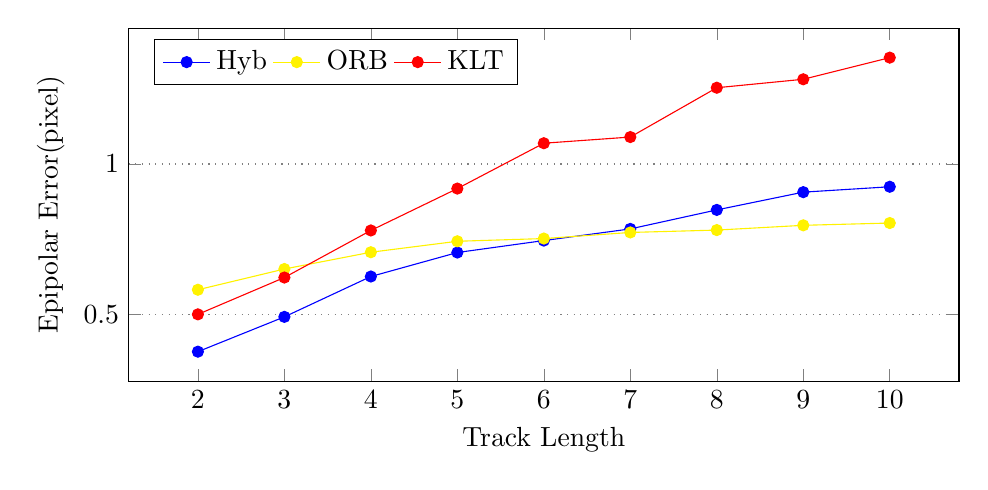
\begin{tikzpicture}
        \begin{axis}[
            xlabel={Track Length},
            ylabel={Epipolar Error(pixel)},
            legend pos=north west, % 图例位置
            legend columns=3, % 设置图例的列数为3
            grid=both, % 显示网格
            major grid style={dotted,gray}, % 主要网格线样式
            minor grid style={dotted,gray}, % 次要网格线样式
            xmajorgrids=false, % 不显示垂直主要网格线
            xminorgrids=false, % 不显示垂直次要网格线
            width=\linewidth, % 宽度设置为12厘米
            height=0.5\linewidth, % 高度设置为4厘米
            ]
            \addplot[color=blue,mark=*] coordinates {
                (2,0.374883)
                (3,0.490805)
                (4,0.625229)
                (5,0.705148)
                (6,0.744951)
                (7,0.783779)
                (8,0.84706)
                (9,0.906202)
                (10,0.924143)
                % (11,0.989535)
                % (12,0.973194)
                % (13,1.139)
                % (14,1.08904)
                % (15,1.14394)
                % (16,1.21185)
                % (17,1.10777)
                % (18,1.4823)
                % (19,1.19149)
                % (20,1.44675)
                % (21,1.43161)
                % (22,1.44882)
                % (23,1.50112)
                % (24,1.52332)
                % (25,1.5785)
            };
            \addlegendentry{Hyb}
            \addplot[color=yellow,mark=*] coordinates {
                (2,0.581117)
                (3,0.650189)
                (4,0.706101)
                (5,0.7426)
                (6,0.751624)
                (7,0.771983)
                (8,0.779857)
                (9,0.79575)
                (10,0.803329)
                % (11,0.808082)
                % (12,0.803262)
                % (13,0.79011)
                % (14,0.798317)
                % (15,0.779228)
                % (16,0.836509)
                % (17,1.0089)
                % (18,0.964484)
                % (19,0.840002)
                % (20,0.889293)
                % (21,0.769063)
                % (22,1.06872)
                % (23,0.855994)
                % (24,1.00139)
                % (25,1.0281)
            };
            \addlegendentry{ORB}
            \addplot[color=red,mark=*] coordinates {
                (2,0.499181)
                (3,0.62185)
                (4,0.778618)
                (5,0.918091)
                (6,1.06917)
                (7,1.08973)
                (8,1.25399)
                (9,1.28214)
                (10,1.35425)
                % (11,1.32911)
                % (12,1.45214)
                % (13,1.39665)
                % (14,1.56813)
                % (15,1.68793)
                % (16,1.74085)
                % (17,1.70084)
                % (18,1.73148)
                % (19,1.64343)
                % (20,1.60756)
                % (21,1.72251)
                % (22,1.91925)
                % (23,2.00618)
                % (24,2.09104)
                % (25,1.83422)
            };
            \addlegendentry{KLT}
        \end{axis}
    \end{tikzpicture}
    \caption{Epipolar error statistics on all data from EuRoC. The x-axis represents track length, and the y-axis indicates the median value of the epipolar error corresponding to the track length.}
    \label{fig:Epipolar_Error}
\end{figure}

% \begin{figure}
%     \centering
% \label{Track-Length}
%     \includegraphics[width=1\linewidth]{pictures/Track-Length.png}
%     \caption{Track length statistics for different sequences in EuRoC.}
%     \label{fig:track-length}
% \end{figure}

\begin{figure}[h]
    \centering
    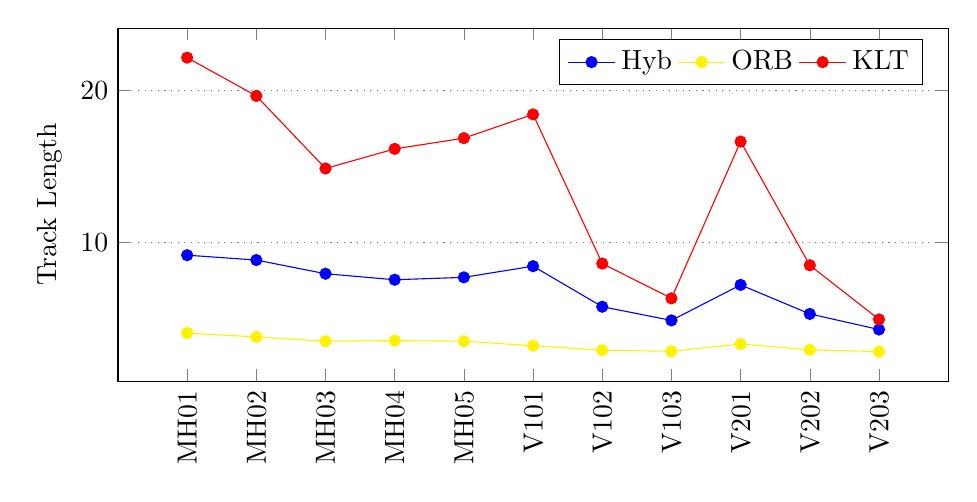
\begin{tikzpicture}
        \begin{axis}[
            % xlabel={Dataset},
            ylabel={Track Length},
            legend pos=north east, % 图例位置
            legend columns=3, % 设置图例的列数为3
            grid=both, % 显示网格
            major grid style={dotted,gray}, % 主要网格线样式
            minor grid style={dotted,gray}, % 次要网格线样式
            xmajorgrids=false, % 不显示垂直主要网格线
            xminorgrids=false, % 不显示垂直次要网格线
            width=\linewidth, % 宽度设置为12厘米
            height=0.5\linewidth, % 高度设置为4厘米
            xtick=data, % 使用数据点的值作为横坐标刻度
            xticklabels={MH01, MH02, MH03, MH04, MH05, V101, V102, V103, V201, V202, V203}, % 设置横坐标的标签
            xticklabel style={rotate=90,anchor=east,xshift=0cm}, % 标签旋转为垂直,锚点为东
            ]
            \addplot[color=blue,mark=*] coordinates {
                (1,9.16401)
                (2,8.84333)
                (3,7.94203)
                (4,7.54585)
                (5,7.70342)
                (6,8.44075)
                (7,5.76857)
                (8,4.86837)
                (9,7.20563)
                (10,5.2953)
                (11,4.26726)
            };
            \addlegendentry{Hyb}
            \addplot[color=yellow,mark=*] coordinates {
                (1,4.03109)
                (2,3.77664)
                (3,3.49368)
                (4,3.53465)
                (5,3.49801)
                (6,3.19997)
                (7,2.90238)
                (8,2.83099)
                (9,3.3095)
                (10,2.93061)
                (11,2.80861)
            };
            \addlegendentry{ORB}
            \addplot[color=red,mark=*] coordinates {
                (1,22.1775)
                (2,19.655)
                (3,14.8748)
                (4,16.1651)
                (5,16.8731)
                (6,18.4386)
                (7,8.61279)
                (8,6.32001)
                (9,16.6511)
                (10,8.50012)
                (11,4.93324)
            };
            \addlegendentry{KLT}
        \end{axis}
    \end{tikzpicture}
    \caption{Track length statistics for different sequences in EuRoC. Y-axis indicates the mean track length of each sequence.}
    \label{fig:track-length}
\end{figure}

To assess the effectiveness of the hybrid matching method, we conducted a comparative analysis using different matching strategies on the EuRoC dataset. These strategies include ORB's KNN matching, optical flow matching and hybrid matching. 

To evaluate the accuracy of feature matching, we employed the epipolar error metric. Using the true pose values provided by the dataset, we computed the relative pose between the two matched frames. Subsequently, with the relative pose and intrinsic parameters, we derived the fundamental matrix. The epipolar error metric is then calculated using the epipolar geometric relationship as follows:
\begin{equation}
        E_{epi} = \textbf{p}_i^T \textbf{F} \textbf{p}_j,
\end{equation}
where $\textbf{F}$ represents the fundamental matrix between frame $i$ and frame $j$ ,  and $\textbf{p}_i,\textbf{p}_j$ denote the corresponding feature points on the two frames.
We analyzed the relationship between track length and epipolar error across different feature matching methods using the entire EuRoC dataset. Specifically, \textit{ORB} denotes continuous frame KNN matching based on ORB features, \textit{KLT} signifies the optical flow method, and \textit{Hyb} represents our proposed hybrid method. From the results depicted in \cref{fig:Epipolar_Error}, it is observed that as the track length increases, the epipolar error also increases, indicating a positive correlation trend. Descriptor-based matching exhibits the smallest epipolar error, while optical flow-based matching demonstrates the largest epipolar error. Our hybrid matching method lies between them. Compared with optical flow matching, the hybrid method demonstrates a significant improvement in matching accuracy.

We further conducted statistical analysis on the track length of different matching strategies. In \cref{fig:track-length}, we observe that the optical flow-based method consistently yields longer track lengths across all sequences. However, these lengths exhibit significant fluctuations with changes in scene and movement speed. Additionally, as shown in \cref{fig:Epipolar_Error},  the long tracks produced by the KLT method may result in large epipolar errors, thereby not contributing to accuracy improvement. Our hybrid method maintains a moderate track length and exhibits stability across different sequences. Compared to the descriptor-based method, the track length of the hybrid approach shows a significant increase, nearly doubling.

We also compared the time consumption of the hybrid method and the KLT method in \cref{tab:time_statistics}. Despite the hybrid method utilizing both ORB and KLT in feature matching, the overall time consumption does not increase significantly. This is attributed to the shared feature detection module of ORB and KLT within the hybrid method, with the time-consuming increase primarily occurring in the matching process. Furthermore, leveraging the prior knowledge of KLT eliminates the need to extract an excessive number of ORB points (in our case, only 150 points are extracted), which proves adequate for matching within the sliding window. The time cost of \textit{others} includes triangulation, EKF filter, etc. 
\subsection{Trajectory Evaluation}
\begin{table*}[h]
    \caption{ATE (m)  of different algorithms on EuRoC.  Bold font indicates the best result in each column. '-' represents failure to run on this data. All results (except for HybVIO, whose ATE is obtained from \cite{hybvio}) were obtained by ourselves using open-source code and default configurations. None of them incorporate loop closure. }
    \centering
    \begin{tabular}{ccccccccccccc}
    \toprule
         & MH-01 & MH-02 & MH-03 & MH-04 & MH-05 & V1-01 & V1-02 & V1-03 & V2-01 & V2-02 & V2-03 & Avg. \\
         \midrule
         OKVIS      & 0.337 & 0.306 & 0.253 & 0.305 & 0.392 & 0.090 & 0.145 & 0.255 & 0.234 & 0.163 & 0.242 & 0.247 \\
         VINS-Mono  & 0.155 & 0.178 & 0.224 & 0.344 & 0.293 & 0.089 & 0.112 & 0.180 & 0.082 & 0.129 & 0.307 & 0.190 \\
         VINS-Fusion& 0.181 & 0.092 & 0.167 & 0.203 & 0.304 & 0.064 & 0.270 & 0.158 & 0.082 & -     & 0.160 & 0.168 \\
         OpenVINS   & \textbf{0.079} & 0.149 & 0.138 & 0.204 & 0.502 & 0.061 & 0.063 & \textbf{0.063} & 0.101 & \textbf{0.064} & 0.178 & 0.146 \\
         HybVIO     & 0.190 & \textbf{0.066} & \textbf{0.120} & 0.210 & 0.310 & 0.069 & 0.061 & 0.080 & \textbf{0.052} & 0.089 & 0.130 & 0.130 \\
         \midrule
         XR-VIO(KLT)& 0.106 & 0.144 & 0.145 & 0.230 & \textbf{0.212} & \textbf{0.050} & 0.044 & 0.100 & 0.073 & 0.071 & 0.158 & 0.121 \\
         XR-VIO(ORB)& 0.164 & 0.140 & 0.204 & 0.354 & 0.309 & 0.124 & 0.107 & 0.201 & 0.064 & 0.186 & 0.200 & 0.186 \\
         XR-VIO     & 0.082 & 0.114 & 0.164 & \textbf{0.181} & 0.215 & 0.060 & \textbf{0.041} & 0.075 & 0.062 & 0.081 & \textbf{0.100} & \textbf{0.107} \\
         \bottomrule
    \end{tabular}
    \label{tab:ATE_Compare}
\end{table*}
\begin{table*}[h]

    \caption{ATE (mm)  of different algorithms on the ZJU-Sensetime dataset. Bold font indicates the best result in each column. '-' represents failure to run on this data. XR-VIO (KLT) is the ablation version of our XR-VIO, utilizing only KLT for feature matching.}
    \centering
    \begin{tabular}{cccccccccc}
    \toprule
         &  A0&  A1&  A2&  A3&  A4&  A5&  A6&  A7& Avg.\\
         \midrule
         OKVIS\protect\footnotemark[1]          &  71.677 & 87.730 & 68.381 & 22.949 &  146.890 & 77.924 & 63.895 & 47.465 & 73.364 \\
         VINS-Mono\protect\footnotemark[1]      &  63.395 & 80.687 & 74.842 & 19.964 & 18.691 & 42.451 & 26.240 &  18.226 & 43.062 \\
         Vins-Fusion\protect\footnotemark[3]&  77.200 & 134.112 & 40.739 & 23.901 & 28.915 & 57.254 & 26.840 & 25.174 & 51.767\\
         OpenVINS\protect\footnotemark[3]& 74.368 & 97.339 & 41.610 & 22.387 & 16.862 & -   & 22.828 & 15.350 & 41.534\\
         HybVIO\protect\footnotemark[2]         &  \textbf{49.900}&  \textbf{30.000 }&  36.000&  22.200&  19.600&  37.800&  29.300&  17.300& 30.300\\
         SenseSLAM(V1.0)\protect\footnotemark[1]&  58.995 & 55.097 & 36.370 & 17.792 & 15.558 & 34.810 & 20.467 & \textbf{10.777} & 31.233\\
\hline
         XR-VIO(KLT)\protect\footnotemark[3]    &  \phantom{1}60.385\phantom{1} &  \phantom{1}71.926\phantom{1} &  \phantom{1}31.134\phantom{1} &  \phantom{1}16.657\phantom{1} &  \phantom{1}25.913\phantom{1} &  \phantom{1}34.288\phantom{1} &  \phantom{1}20.410\phantom{1} &  \phantom{1}13.125\phantom{1} & \phantom{1}34.230\phantom{1} \\
         XR-VIO(ORB)\protect\footnotemark[3]& 71.694 & 66.478 & 45.526 & 17.621 & 31.178 & 48.582 & 20.355 & 22.422 & 40.482\\
        XR-VIO\protect\footnotemark[3]          &  56.604 &  46.219 & \textbf{30.422} & \textbf{15.291}& \textbf{15.078}&  \textbf{30.283}& \textbf{17.082}&  12.598 & \textbf{27.947}\\
        \bottomrule
    \end{tabular}
    
    \label{tab:ATE_ZJU}
       \footnotemark[1]{ATE is obtained from \cite{jinyu2019survey}  }
       \footnotemark[2]{ATE is obtained from \cite{hybvio} }
       \footnotemark[3]{ATE is obtained by ourselves.}
\end{table*}

In \cref{tab:ATE_Compare,tab:ATE_ZJU}, we respectively compared our approach with the current state-of-the-art \cite{leutenegger-ijrr-2015-OKVIS, qin-tro-2018_VINS-Mono, qin2019a_VINS_Fusion_Local, geneva2020openvins,hybvio} on the EuRoC benchmark and the ZJU-Sensetime benchmark.
% \textit{All of these methods and our own run on same environment. Trajectories are without initialization part.}
% Our approach yields state-of-the-art performance on each dataset.
We also compared our own method with a baseline version employing solely KLT and ORB methods for feature matching, illustrating  the efficiency of our hybrid feature matching. The results demonstrate a noticeable improvement in ATE on both the EuRoC and ZJU-Sensetime datasets.

The ZJU-Sensetime dataset comprises data from consumer-grade mobile phones, captured with rolling cameras resulting in low-quality images often affected by motion blur. As a result, the accuracy of most algorithms is notably reduced when applied to this dataset. Our hybrid matching strategy demonstrates its advantage, particularly under the conditions present in the mobile phone dataset. Optical flow-based methods are particularly sensitive to variations in image quality, with rapid motion or changes in brightness causing significant errors in feature matching. However, our hybrid matching strategy effectively mitigates these issues, thereby improving the accuracy of VIO.
Additionally, more experimental results for accuracy comparison, such as evaluation on ADVIO \cite{cortes2018advio} dataset, can be found in our supplementary material.

In addition to the methods outlined in \cref{tab:ATE_Compare,tab:ATE_ZJU} , we refrain from comparing several other VIO/VI-SLAM systems, such as VI-ORB \cite{murartal-ral-2017-VI-ORB}, ORB-SLAM3 \cite{campos2021orb-slam3}, VI-DSO \cite{von2018direct-VI-DSO}, DM-VIO \cite{stumberg22DM-VIO}, despite their demonstrated high accuracy. This decision stems from their inherent latency issues, rendering them unsuitable for XR applications Latency manifests in two main aspects. Firstly, there is the computational burden. While algorithms in the ORB-SLAM series offer good accuracy, they rely on a significant number of complex calculations, making deployment on mobile platforms challenging. Secondly, there are delays inherent in the algorithm mechanisms. For instance, the ORB-SLAM\cite{murartal-ral-2017-VI-ORB, campos2021orb-slam3} series require 15 seconds of data to complete initialization, and DSO \cite{von2018direct-VI-DSO, stumberg22DM-VIO} series, with delayed marginalization, also need 2\textasciitilde10 seconds to obtain real scale. These latency issues are unacceptable for XR users.
\subsection{Ablation Study}
We conducted an ablation study on each initialization module under the 4KF configuration, as presented in \cref{tab:Ablation}. This analysis aimed to assess the individual impact of each module on initialization performance. The left column lists different algorithm strategies. \textit{Full} denotes our complete strategy for initialization, where all indicators demonstrate the best performance. Subsequently, we examined various ablation strategies. The ablation of \textit{2-point} demonstrates an improvement in the success rate of initialization. This method, when combined with known rotation, simplifies the solution for the initial relative pose. In contrast, the \textit{5-point} method requires solving complex polynomial problems and selecting the correct solution from a candidate set. \textit{VG-BA} represents an enhancement of traditional Visual-BA. By incorporating the orientation constraint of the gyroscope, the solution of the entire SfM problem becomes less prone to divergence, especially in cases of small motion and parallax. Moreover, VG-BA improves the accuracy of orientation estimation by optimizing gyroscope bias. Following VG-BA and initial visual-inertial alignment, the overall VI-BA plays a crucial role. The last two rows of \cref{tab:Ablation} demonstrate the impact of missing complete or partial VI-BA on initialization accuracy. Without VI-BA, scale error significantly increases, highlighting the importance of the weighting of visual terms.
\begin{table}[h]
    \centering

    \caption{Ablation study for VI-Initialization. Bold font indicates the best result, and Italic font highlights significant impact resulting from ablation.}
    \begin{tabular}{ccccc}
    \toprule
          &  Scale(\%)$\downarrow$&  ATE(m)$\downarrow$&  Gravity(°)$\downarrow$&  Succ(\%)$\uparrow$\\
          \midrule
           Full&  \textbf{26.88}&  \textbf{0.026}&  \textbf{2.26}&  \textbf{83.98}\\
           w/o 2-point&  27.08&  0.027&  2.34&  \textit{\textbf{80.43}}\\
           w/o VG-BA&  26.92&  0.027&  \textit{\textbf{2.45}} &  82.62\\
           w/o VI-BA&  \textit{\textbf{30.68}}&  0.028&  2.37&  83.98\\
          w/o weight&  \textit{\textbf{28.27}}&  0.028&  2.30&  83.84\\
    \bottomrule
    \end{tabular}
    \label{tab:Ablation}
\end{table}

\subsection{Mobile AR}
%We deployed our VIO system to mobile platforms (Android \& iOS) and developed a simple AR demo to demonstrate its accuracy and robustness. We utilized 30 Hz image data with a resolution of $640\times480$ and IMU data, including angular velocity and acceleration captured at 100/200Hz by the iPhone 13 Pro and Huawei Mate30 Pro. Our system operates in real-time on mobile devices, seamlessly integrating virtual objects into real-world scenes. \cref{fig:fancy AR demo} shows two AR examples. We assessed the accuracy of the algorithm by examining loop errors in the 3D trajectory during long-distance motion tracking in expansive scenes. Over tracking distances of several hundred meters, no visually significant loop errors or height discrepancies were observed. The experimental results demonstrate the superiority of our system in both initialization and normal tracking tasks, highlighting the effectiveness of our algorithm in XR applications. Further details of our mobile AR implementation can be found in our supplementary video material.
We deployed our VIO system on mobile platforms (Android \& iOS) and created a simple AR demo to showcase its accuracy and robustness. Using 30 Hz image data at a resolution of 640×480 and IMU data, including angular velocity and acceleration captured at 100/200Hz by the iPhone 13 Pro and Huawei Mate30 Pro, our system operates in real-time on mobile devices. It seamlessly integrates virtual objects into real-world scenes. \cref{fig:fancy AR demo} displays two AR examples. We evaluated the algorithm's accuracy by examining loop errors in the 3D trajectory during long-distance motion tracking in large scenes. Over distances of several hundred meters, no significant loop errors or height discrepancies were visually observed. The experimental results highlight the system's superior performance in both initialization and normal tracking tasks, emphasizing the algorithm's effectiveness in XR applications. Additional details of our mobile AR implementation are available in our supplementary video material.
\begin{figure}
    \centering
    \includegraphics[width=\columnwidth]{pictures/Mobile-AR.png}
    \caption{AR effects on mobile platforms}
    \label{fig:fancy AR demo}
\end{figure}
% \begin{figure}
%     \centering
%     \includegraphics[width=1\columnwidth]{pictures/Mobile-Trajectory.png}
%     \caption{Trajectory of VIO on a mobile phone: \textcolor{red}{need to add pic @nan, online AR + Trajectory}.}
%     \label{fig:fancy AR demo}
% \end{figure}
